% TEMPLATE for Usenix papers, specifically to meet requirements of
%  USENIX '05
% originally a template for producing IEEE-format articles using LaTeX.
%   written by Matthew Ward, CS Department, Worcester Polytechnic Institute.
% adapted by David Beazley for his excellent SWIG paper in Proceedings,
%   Tcl 96
% turned into a smartass generic template by De Clarke, with thanks to
%   both the above pioneers
% use at your own risk.  Complaints to /dev/null.
% make it two column with no page numbering, default is 10 point

% Munged by Fred Douglis <douglis@research.att.com> 10/97 to separate
% the .sty file from the LaTeX source template, so that people can
% more easily include the .sty file into an existing document.  Also
% changed to more closely follow the style guidelines as represented
% by the Word sample file. 

% Note that since 2010, USENIX does not require endnotes. If you want
% foot of page notes, don't include the endnotes package in the 
% usepackage command, below.

% This version uses the latex2e styles, not the very ancient 2.09 stuff.
\documentclass[letterpaper,twocolumn,10pt]{article}
\usepackage{usenix,epsfig,endnotes}
\begin{document}

%don't want date printed
\date{}

%make title bold and 14 pt font (Latex default is non-bold, 16 pt)
\title{\Large \bf Scalable Crowd-sourced Live Streaming System}

%for single author (just remove % characters)
\author{
{\rm Anbang Zhao}\\
Carnegie Mellon University\\
5000 Forbes Ave\\
Pittsburgh, PA 15213, USA\\
anbangz@cs.cmu.edu
\and
{\rm Zhuo Chen}\\
Carnegie Mellon University\\
5000 Forbes Ave\\
Pittsburgh, PA 15213, USA\\
zhuoc@cs.cmu.edu
% copy the following lines to add more authors
\and
{\rm Mahadev Satyanarayanan}\\
Carnegie Mellon University\\
5000 Forbes Ave\\
Pittsburgh, PA 15213, USA\\
satya@cs.cmu.edu
} % end author

\maketitle

% Use the following at camera-ready time to suppress page numbers.
% Comment it out when you first submit the paper for review.
\thispagestyle{empty}


\subsection*{Abstract}

We propose a scalable system for Internet scale crowd-sourced live streaming video broadcasting from wearable devices, like Google Glass and smart watches. Instead of the widely used centralized system architecture which inevitably face single point bottlenecks, our approach uses a decentralized architecture on cloudlets. We construct an overlay tree on top of cloudlets connected via wide area network (WAN) and do application layer multicast (ALM) on those nodes which effectively reduced bandwidth consumption from linear to client number to linear to cloudlet number. Furthermore, to make this system work, each cloudlet node can just send one copy of the stream, which effectively solves the single node bottleneck. In the Internet scale, there might be hundreds or thousands of cloudlets serving the same stream, our system can tolerate possible cloudlet failures and reconstruct the tree structure within a short period of time. Our experiments show that our system can effectively reduce bandwidth consumption on WAN and keep the same video quality.

\subsection*{Keywords}

mobile computing, application layer multicast, cloud computing, cloudlet, Google Glass

\section{Introduction}

Wearable devices with a camera on it has becoming more and more popular over the past years. Go Pro sold 2.3 million devices in the year of 2012 and Go Pro users can easily upload their Go Pro videos to their favorite video websites (e.g. YouTube) through their mobile devices. Google launched the famous Google Glass in 2012 and it soon became a star in the technology world. Galaxy Gear and Apple Watch are more recent such kind of products that draw much attention from the world. With these kind of technology products, to capture and broadcast a first-person viewpoint video just requires the user to press a button or touch the screen. People can do what they intend to do without interferencec brought by wearing those devices and doing video capturing. A good example of this is the first-person hiking videos captured by Go Pro on YouTube. They have good resolution and gives viewers a better experience. Another example is JustinTV, which turned into Twitch and was aquired by Amazon with 1 billion dollars. It was famous for providing first-person videos of good game players and people love to watch it.

\begin{figure}[t]
\begin{center}
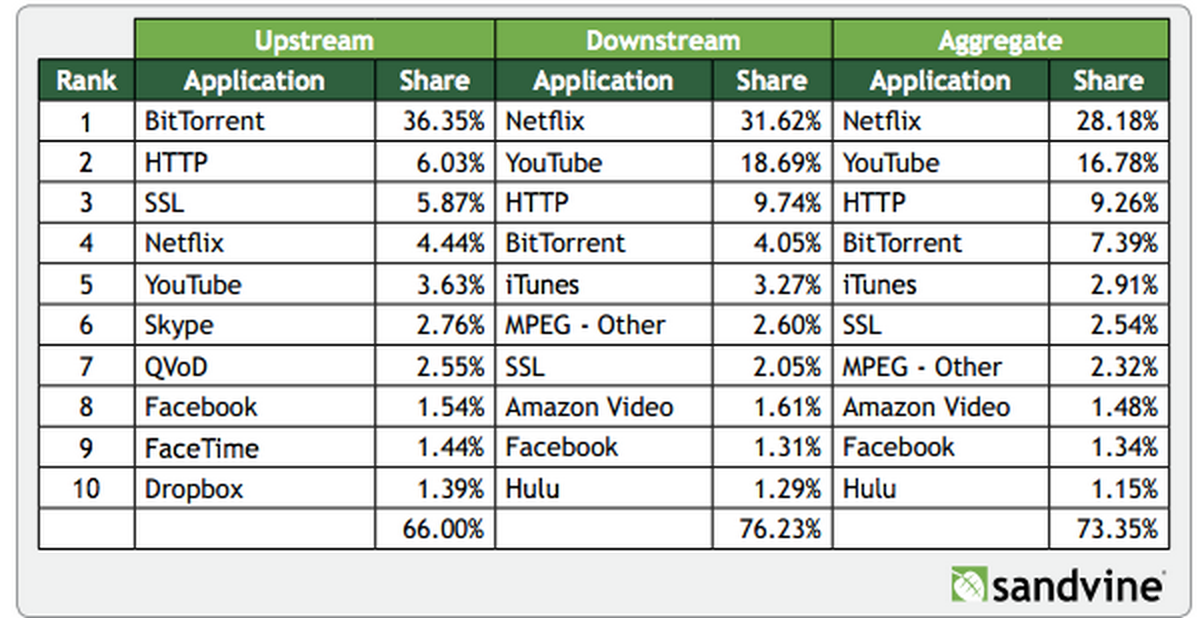
\includegraphics[scale=0.3]{pic/bandwidth_rank.png}
\end{center}
\caption{US bandwidth consumption (from sandvine)}
\end{figure}

We believe video broadcasting is the more intuitive and vivid way of communication and emotion sharing and more and more people will use this kind of service. But this service comes with a big price, Internet bandwidth in both uploading and downloading. Video stream is already the biggest consumer on the Internet. As shown in Figure 1, Netflix and Youtube consume about half the downloading bandwidth in the US. We can anticipate an even greater download bandwidth consumption if those live streaming videos are available. Besides, the upload bandwidth consumption will increase even more than the download bandwidth consumption. Currently, uploading video is not much more troublesome than watch a video. However, in the near future, it will become as easy because of the all the smart hardwares. At that time, the bandwidth bottleneck of the current video system will be more severe because content distribution network (CDN) will not help neither. 



\begin{figure}[h]
\begin{center}
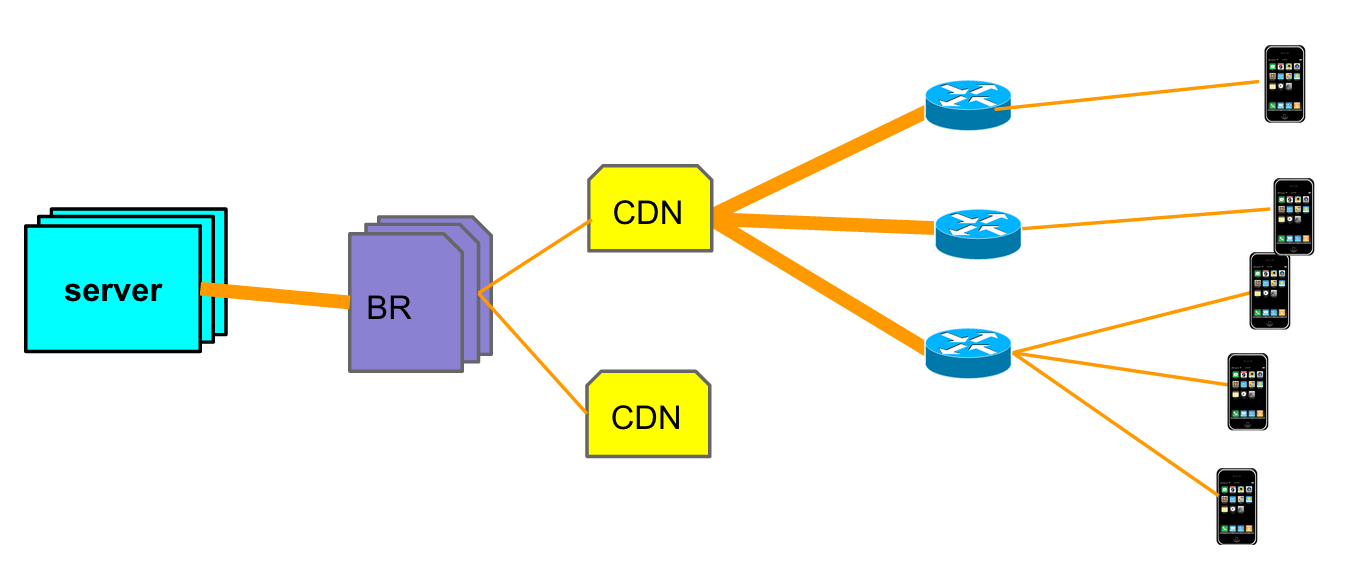
\includegraphics[scale=0.3]{pic/central_archi.png}
\end{center}
\caption{centralized video system architecture}
\end{figure}

However, current video systems are not optimized for the ever increasing bandwidth consumption. Current video streaming systems mostly use the centralized architecture as shown in Figure 2. In this architecture, the same copy of data will be transmitted over WAN for multiple times even when two clients are very close to each other. WAN bandwidth is not properly utilized. Besides, the central server or a CDN server may be overwhelmed by a large demand. 

The problems existing in the centralized server lead us to think if we can build a decentralized video system. And we do find two good opportunities. The first one is that bandwidth is very large now for both wired LAN and wireless LAN. Wired LAN is known to be very fast for a long time. For wireless LAN, the recently approved 802.11 ac protocol has a maximum bandwidth of about 1300 Mbps, which is a significant improvement from its predecessors. Large available LAN bandwidth means that we do not need to worry about the last hop communication. All we need to care about is how to effectively transmit video streams from the source to the local access point. The other opportunity comes from cloudlets~\cite{simoens2013scalable}. Cloudlet is attached to the local access point (AP) and has reasonable computation power. Because it's attached to AP, all the clients can communicate with the cloudlets via LAN. With its computation power, we can dynamically do adaptations to better serve videos based on the current network conditions. These two features make cloudlet the best fit to build an application layer multicast system.

In this paper, we propose a new decentralized video streaming system. In our system, there is no central streaming server. All the cloudlets are connected with cloudlets via LAN. All the cloudlets are connected with other cloudlets via WAN. We have a central metadata server to manage the overlay tree structure of the cloudlets. Only control data are transmitted between cloudlets and metadata server so that it will not have a bandwidth bottleneck in the metadata server. By doing ALM, we effectively reduces bandwidth consumption from linear to client number to linear to cloudlet number. Because of the ample LAN bandwidth and reasonable computation power on cloudlets, one cloudlet can server tens of cloudlets. Thus, our system can reduce bandwidth consumption by an order of magnitude in the best situation. This paper makes the following contributions:

\begin{itemize}
  \item It describes the benefits of a live streaming system on the new wearable devices, identifies the technical challenges in scaling such a system, and analyzed why the current architecture cannot satisfy a huge demand in the future.
  \item It proposes a new decentralized architecture to do Internet scale live streaming broadcast. This architecture is built on top of cloudlets and achieves scalability by using ALM to reduce bandwidth consumption on WAN and solve the single point bottleneck. It describes the tradeoffs in the design process.
  \item It builds a running system on cloudlets and Google AppEngine. It includes the server codes on cloudlet, metadata code on Google AppEngine and client code on Google Glass. The client code is used just used for a demo. As we make no assuptions on clients, developpers can easily build their own client and use our service. This whole project is open sourced to all that are interested in this work.
  \item It evaluates the system on its scalability, bandwidth efficiency, video quality and fault tolerance.  
\end{itemize}

Section 2 describes the overall architecture of our decentralized live straming system. Section 3 describes the design of the cloudlet server which are effectively streaming servers on cloudlets. Section 4 describes the design and implementation of the metadata server which manages the overlay tree structure. Section 5 describes the fault tolerance mechanism of the system and tradeoffs in the design space. Section 6 has performance measurements of the implemented system on different configurations. Section 7 discusses related and future work. Section 8 is the acknowledgements. Section 9 describes where and how to get the source code of the system.

\section{System Architecture}

\subsection{System Goals}
Our goal is to build a scalable live streaming system. To be more specific, it has two major goals:

\begin{enumerate}
  \item Our system should be scalable for stream uploading
  \item Our system should be scalable for stream downloading
\end{enumerate}

We specifically split stream downloading and uploading because most of the current systems and researches only focus on stream downloading. And we believe, with more and more wearable devices which could conveniently upload streams, stream uploading would be a bottleneck as well.

Except for those two major goals, we also have two additional bonus goals:
\begin{enumerate}
  \item A smaller latency would be better
  \item A smaller control traffic is better
\end{enumerate}

Smaller latency is better but we don’t require that the latency should be very small. Our live streaming system is not meant to be an interactive system. So when we need to make a tradeoff between latency and bandwidth, we would pick bandwidth. 

The same goes to control data. Smaller control data would reduce the response time and save bandwidth. However, control data is quite smaller compared with streaming data. So we would not emphasize on control data. 

Besides, the system requirements, we also have some features to use to build the system. Taking advantage of these features makes our system much easier to design and better serve the requirements. The good thing is that we are building a live streaming system. Live streaming could give us the below benefits in building our system.

\begin{enumerate}
  \item Data is live streamed. There’s no need to store data.
  \item All the clients are actually requesting the same data. Unlike on-demand videos, people may be viewing the same video at different time. For live streaming, people are always watching the current time.
\end{enumerate}

No data needs to be stored. This gives us the opportunity to build a fully distributed system. We don’t need a central server to store the data. Central server would always be a bottleneck and without it we could build a fully distributed scalable live streaming system.

All clients are requesting the same data. So we don’t need to get different data from different clients in the peer-to-peer scheme. We could randomly pick a peer and that data must be the data this client is requesting. This makes our scheme much easier.

\subsection{Overlay Forest}

Our system is an Internet scale decentralized video steaming system. As shown in Figure 3, we build an overlay forest on top of the WAN. The nodes in the forest are cloudlets. The green line means WAN stream data. The blue line represents LAN stream data and the dotted line is WAN communication data. So we can see that cloudlets connect with other cloudlets via WAN. The root of a single tree (blue nodes in the forest) is the cloudlet that acts as the stream sender. The forest and tree structure is managed by a metadata server. All the clients communicate with cloudlets via LAN. This is not part of our overlay forest because oud system only cares about WAN communications. 

\begin{figure}[t]
\begin{center}
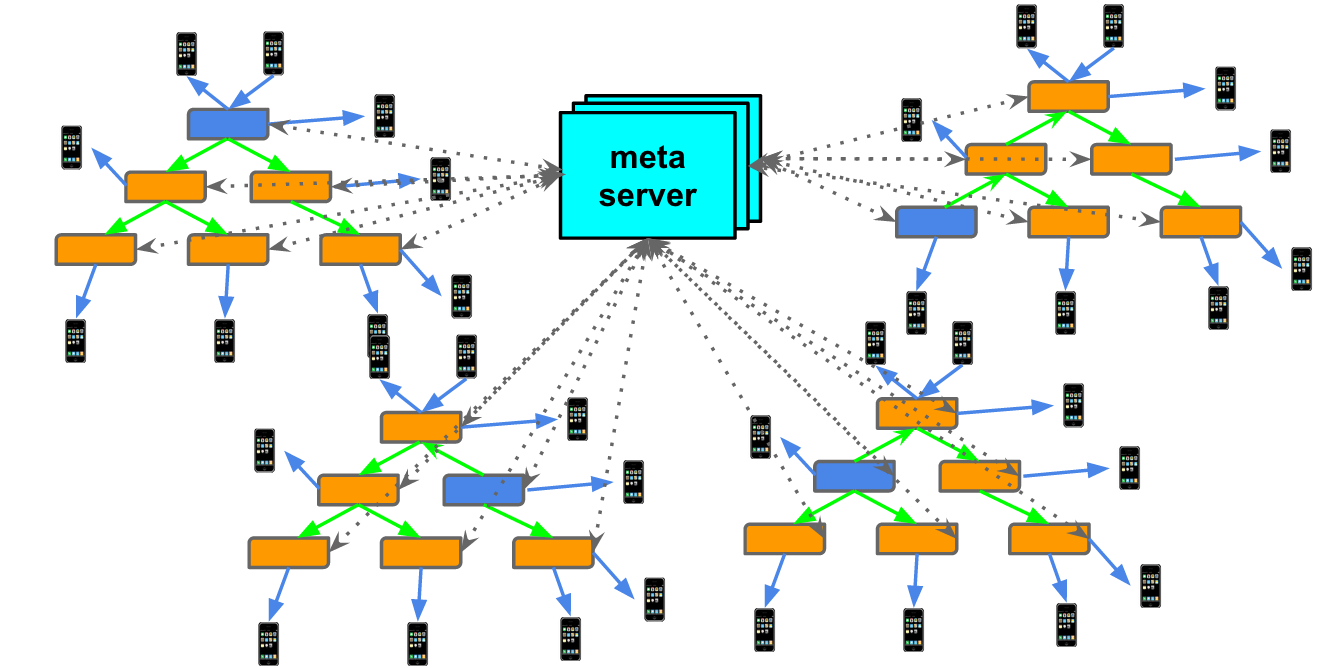
\includegraphics[scale=0.3]{pic/overlay_forest.png}
\end{center}
\caption{system architecture}
\end{figure}

\begin{figure}[h]
\begin{center}
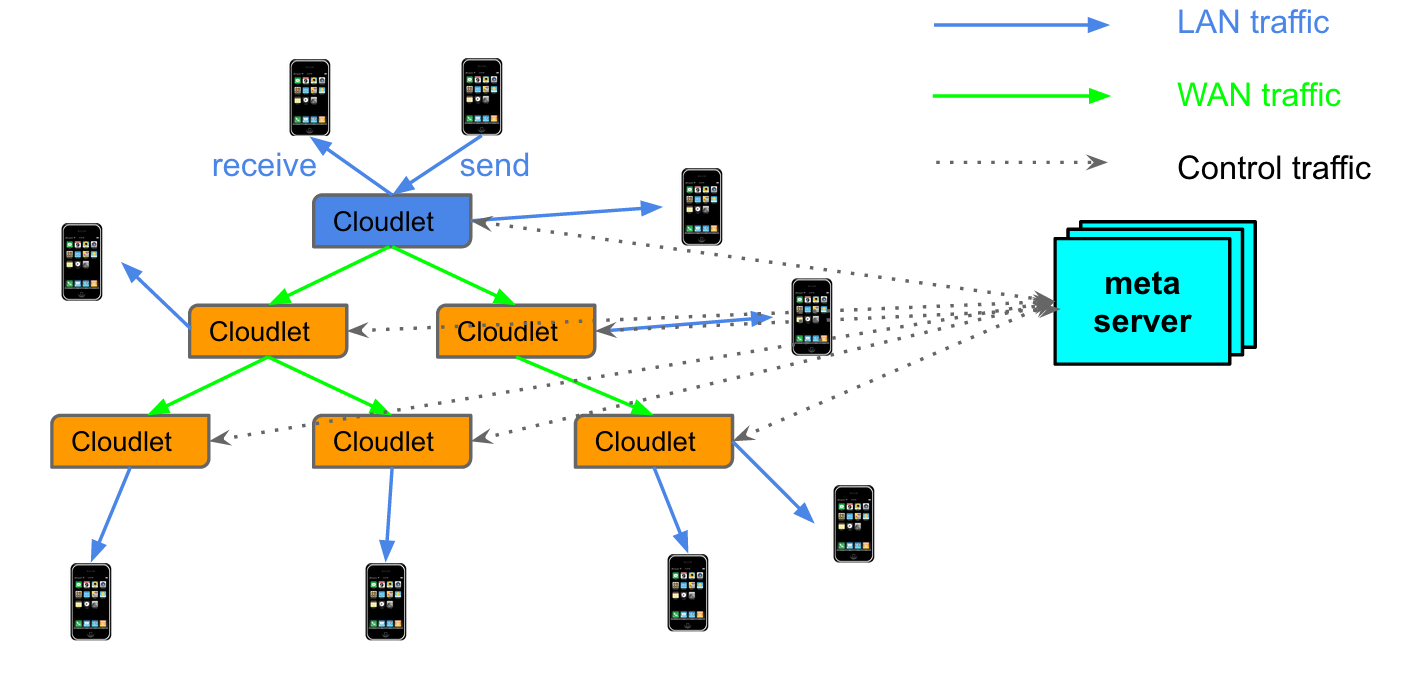
\includegraphics[scale=0.3]{pic/overlay_tree.png}
\end{center}
\caption{overlay tree structure}
\end{figure}

One tree represents one specific stream with one sender and multiple receivers. Our system supports multiple streams with multiple receivers. For each specific stream, the structure and operation are similar. Figure 4 shows one stream in the forest. Each cloudlet could have heterougenious computation power and bandwidth capacities. They will report their current machine status and stream status to the metadata server repeatedly via a heartbeat message and the metadata server will then decide the tree architecture accordingly. 

\begin{figure}[t]
\begin{center}
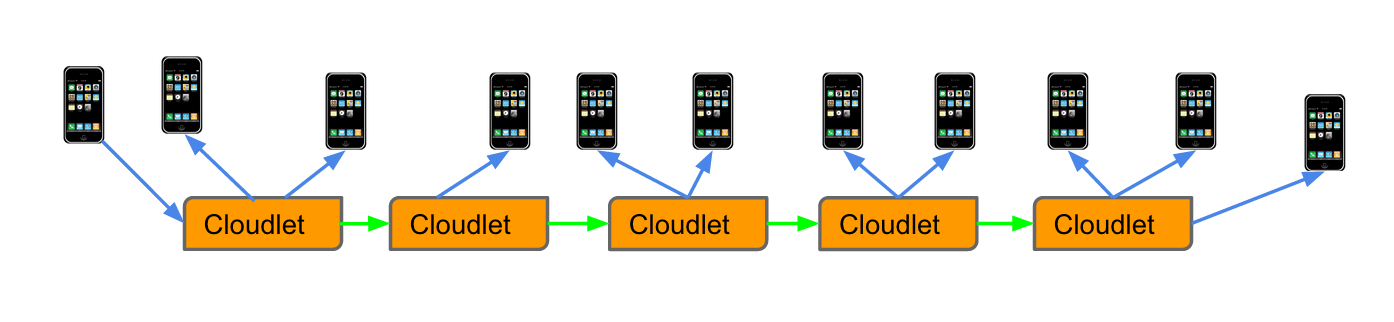
\includegraphics[scale=0.3]{pic/line_structure.png}
\end{center}
\caption{line structured overlay tree}
\label{fig:line_structure}
\end{figure}

Tree structure affects the system performace a lot and each tree structure reconfiguration will take a reasonably long time. So each tree construction decision is made with caution by the metadata server. The tradeoff in the design space here in tree structure is mainly about latency and bandwidth consumption. If we line the cloudlets up in a straight line as shown in Figure~\ref{fig:line_structure}, we will have the smallest bandwidth consumption on WAN. Each cloudlet just needs to send out one copy of data on the WAN. However, the price we take here is the latency. The tail nodes have to wait for all the previous nodes doing buffering and sending it the data it needs. 

\begin{figure}[h]
\begin{center}
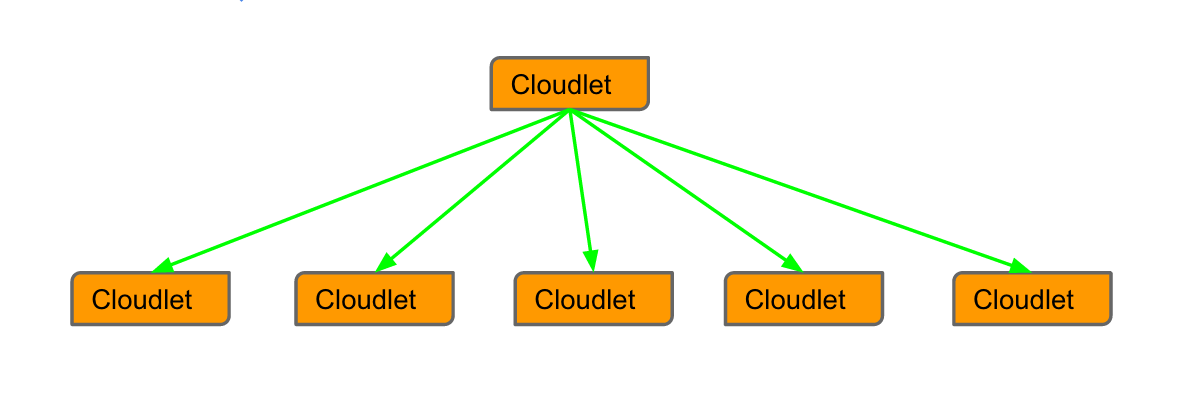
\includegraphics[scale=0.3]{pic/large_fanout.png}
\end{center}
\caption{large fanout structured overlay tree}
\label{fig:large_fanout}
\end{figure}

If we use a structure with large fanout at each node as shown in Figure~\ref{fig:large_fanout}, our decentralized model will degrade to a centralized model when the fanout is big. The same problems with the centralized architecture will come back, although we enjoy a smaller latency here.



\subsection{System Design Assumptions}

Our system makes certain assumptions about the environment our system will be used. They affect our design choinces in later sections. The assumptions are:

\begin{enumerate}
  \item LAN always has ample bandwidth. WAN does not.
  \item Bandwidth is important. Lantecy is not as important.
  \item Clients are not reliable.
  \item Cloudlet can fail. Network could be partitioned but these kind of failures will not occur frequently.
\end{enumerate}

For assumption 1, we have proved that using the current technology parameters. This is the reason why we build our system. For assumption 2, we are building a live streaming broadcasting system, not a video chat system. Latency is not the key factor we are considering now. When there are conflicts between lantecy and bandwidth, we will favor bandwidth. Of course, high latency is not what we want. So we will reduce the latency to the best as long as bandwidth is not sacrificed. For assumption 3, we expect that more and more clients will be mobile and wearable devices that are connected to the Internet via wifi. They are not reliable. They may lose connection at any time. For assumption 4, cloudlet is not like clients. They are servers in a safe box and connected to the Internet with wires. They are less reliable than servers in data centers but are high more reliable than clients.

\section{Cloudlet Server}

\subsection{Server Design}
Cloudlet server is an abstraction of the service provider on cloudlets. It consists of three major components: streaming server, control server and a stream monitor. Streaming server is just an ordinary streaming server. It collects streams from senders and receivers can then get stream data from the stream server. Control server is the core of the cloudlet server. It recieves requests from clients, asks streaming server to open or close a stream and communicates with the metadata server to update stream status. All the control data go to the control server. Stream monitor is a cron job that runs on the cloudlet. It's a bridge between the streaming server and the control server. Control server will get stream status information from the stream monitor rather than the streaming server. This additional layer of indirection makes control server and streaming server independent of each other. It adds flexibility and modularity to our system.

The cloudlet server opens 4 APIs for the clients:

\begin{itemize}
  \item openStream(userName, appName, streamName, streamBandwidth)
  \item closeStream(userName, appName, streamName)
  \item joinStream(userName, appName, streamName)
  \item exitStream(userName, appName, streamName)
\end{itemize}

We first expain the parameters in the APIs. Parameter \emph{userName} is used to identify the user requesting to send or receive a specific stream. It is used to do permission control. Some streams may be private to some particular users. Parameter \emph{appName} and \emph{streamName} is used to identify a specific stream. There can't be two streams with the same appName and streamName. We added the \emph{appName} to make our system more general to support multiple applications. Parameter \emph{streamBandwidth} in the openStream API is used for an estimation of the uploading video. This quality is estimated by clients and sent to the server. Our server may update this value when it finds the real stream bandwidth consumption is different to the estimated value to a big extent.

\emph{openStream} is used for a client to start broadcasting live streaming data. \emph{closeStream} is used for the stream broadcaster to stop serving data. If the client forgot to do that, that's fine. Our system will detect it and call this API. \emph{joinStream} is used by a client to receive a specific stream. \emph{exitStream} is used by a client to exit receiving the stream. Also, it the client forgot to call this API, we will detect it and call it for the client. 

\subsection{Streaming Server}
Our streaming server uses Nginx with rtmp module. Nginx is an open source server. With rtmp module, it can receive and provide stream data in rtmp protocol. Rtmp protocol is widely used in live streaming serving and is also what our system accepts. Nginx with rtmp module supports multiple application and multiple streams. It satisfies our need to be a general live streaming service provider. 

To build a streaming system is hard and needs much knowledge on streaming codec and resource management. That's why we choose to use Nginx with rtmp module. It greatly reduces our development efforts in building the system. However, it do come with some problems. The first one is for buffering. Nginx with rtmp module will require a buffering to recognize the codec of the incoming stream. This is the main source of latency. Secondly, it do provide APIs to get the streaming status in the streaming server. However, to reduce resource consumption, it does so with a fixed length of time. This time is not configurable. This makes our detection of failures take a longer time.

To fully control the incoming stream and connect cloudlets, we use ffmpeg~\cite{tomar2006converting} to create a stream pipe connecting two streaming servers. Ffmpeg is widely used in all kinds of video processing and transmitting jobs. It's open sourced and supports all the common video and audio codec. The price comes with this desigh is also the latency because ffmpeg will do buffering as well.

\subsection{Control Server}
The control server is a http server built with Django. All the control messages from clients and the metadata server will go to this server. The APIs open to the clients are all implemented in the control server.

When a client wants to broadcast live streaming video, it will call the \emph{openStream} API of the control server. Then the server will first check if this user can broadcast the video with the user defined application name and stream name. If it can , the control server will communicate with the metadata server and become a root node of the stream overlay tree in the metadata server. Then the server will tell the client to transmit video data to the stream server and this stream is marked available in the control server.

When a client wants to exit broadcasting live streaming data, it will call the \emph{closeStream} API. Then the control server will tell the metadate server to destroy the stream tree it previously built. Then it tells the streaming server to stop receiving and offering data of this stream and mark this stream as finished in its internal data structure.

When a client wants to watch a stream, it tells the control server by calling the \emph{joinStream} API. Then the control server will first check if it already has this stream available. If so, it direct the client go to the streaming data directly for the stream it wants. If not, it will go to the metadata server to ask for the name of a cloudlet holding the stream data. After getting the cloudlet name, it will create a pipe between the streaming servers on the two cloudlets by using ffmpeg. Then it directs the client to the local streaming server for the stream data.

When a client wants to exit watching a stream, it tells the control server by calling the \emph{exitStream} API. Then the control server will check if there are other clients in the same LAN watching the stream. If so, it does nothing. If not, it tells the metadata server to delete itself from the stream tree and mark the stream in its internal data structure as finished.

The control server also needs to send heartbeat messages to the metadata server to repeatly report the machine status and the stream status. For machine status, it includes current bandwidth consumption and packate loss rate. Streaming server is IO intensive, so we do not send CPU usage or memory usage to the metadata server. Stream status includes bandwidth usage on each stream, number of cloudlets connecting to this cloudlet for the stream and number of clients connected to this cloudlet for this stream.

The control server acts both as client and server. For the real clients, it is a http server. For the metadata server, it acts as a client and send http request to the metadata server. In all of our client-server communications, we use pull strategy. Only client will send requests to the server. The server will never initiate a request to the clients. This simplifies our system design and makes the fault tolerance easier. We will talk more about that in section 5.

\subsection{Stream Monitor}

The stream monitor is a cron job running on the cloudlet. It is a middle layer between the streaming server and the control server. It repeatedly collects stream information from the streaming server by analyzing the statistic file the Nginx server generates and updates. It has two communication channels to the control server. When everything is normal, the stream monitor repeatedly report stream status to control server in a fixed time interval. If it detects anything irregular, it will directly report error to the control server and the control server will decides further actions. This part will be discussed more in section 5 fault tolerance. 

Stream monitors in the system is critically important. It acts as sensors. There may be inconsistency between cloudlet control server and metadata server, and/or inconsistency between control server internal data structure and the real situations. All the final decisions are made based on the information provided by the stream monitor. When any inconsistency is found between the metadata and the information provided by the monitor, the monitor wins and the internal data structure will be corrected.


\section{Metadata Server}

\subsection{Server Design and Implementation}
Metadata server is the most important part in the whole system. It constructs, expands and maintains the overlay tree structure. In case of failures, it's responsible for reconstructing the overlay tree structure. Therefore, we want to make this server extremely available. Besides, all the cloudlets will send heartbeat and other requests to the metadata server. It will not consume large bandwidth but it do impose a the problem of single point failure. So we decided to build this server on Google AppEngine. Google's cloud infrastructure will offer us scalability and reliability. All the servers are stateless. They receive http requests and return http responses. The states of the system is safely stored in the datastore all servers share. Datastore is built on BigTable by Google and has great availability and scalability.

Metadata server opens APIs for cloudlet control servers. Only the control server will call those APIs. They are completely hidden to clients. Those APIs are:

\begin{itemize}
  \item initNode(cloudletName, maxBandwidth)
  \item createTree(cloudletName, appName, streamName, streamBandwidth)
  \item exitTree(appName, streamName)
  \item joinTree(cloudletName, appName, streamName)
  \item heartbeat(cloudletName, cloudletStatus, streamStatus)
\end{itemize}

\emph{initNode} will be called when the cloudlet starts service. It will only be called once. When the metadata server receives this request, it will create a cloudlet data structure to represent the cloudlet which initiates the request. An important parameter of this API is the \emph{streamBandwidth}. It's the maximum bandwidth the cloudlet thinks it has and the metadata server will not break this whenever it has another option.

The control server will call \emph{createTree} when a client requests broadcasting a stream. Metadata server will create an overlay tree rooted on the requesting cloudlet after receive this request.

The control server will make \emph{exitTree} request when the sending client finishes serving data or all the viewers in the same LAN with the cloudlet exited watching. Metadata server will first check the position of the requesting cloudlet in the overlay tree. If it's the root node, it destroys the whole tree. If it's from a non-root cloudlet, it will check whether it's a leaf cloudlet. A leaf cloudlet means that no other cloudlets depend on this cloudlet to get data of this particular stream. If it is a leaf cloudlet, it is safe to exit. If it is not, the metadata will not allow it to exit because once it stops serving the stream data, all its decendents in the subtree rooted on this cloudlet will need to be reconfigured to other cloudlets. This will stop the stream on those cloudlets for about 30 seconds. The metadata server will instead make that cloudlet as a dummy node in the overlay tree structure. The new coming cloudlets will not be scheduled to a dummy node. So the intermediate descendents of that node will never increase. We will exit that node when it becomes a leaf node. 

When a cloudlet has a request from clients asking for a stream it does not have now, it will make a \emph{joinTree} request to the metadata server. The metadata server will respond with the cloudlet name of a cloudlet serving that stream. That cloudlet is chosen by a scheduling algorithm. That algorithm will be described in the next subsection. 

Control server sends \emph{heartbeat} messages to the metadata server with its own status and stream status. This keeps the cloudlet alive in the metadata server. Whenever a cloudlet has not contacted the metadata server for a pre-defined time interval, it will mark this cloudlet as unavailable. New cloudlets will not be scheduled to an unavailable cloudlet. The metadata server will not delete the node representing that cloudlet in the overlay trees because this can best keep the subtree structure. 

\subsection{Scheduling}
Scheduling algorithm determins the overlay tree structure. The tree structure will then affect bandwidth consumption on WAN and latency. Our scheduling algorithm will favor bandwidth to latency as we explained in section 2. The general idea of this algorithm is to search from the root using breadth first search (BFS) to find the first node with enough available bandwidth for serving this stream. We use BFS because we want to find a cloudlet nearest to the root so that it has the smallest latency. In the cases of inconsistency and failures, the algorithm may find the cloudlet requesting to join tree has already been in the tree. In this case, we delete the old node and re-schedule the node to another node in the overlay tree that is not in the subtree rooted on that cloudlet in the old tree configuration. If the algorithm finds that no available nodes are there, it will randomly pick one node to serve the data. The algorithm is shown in the code snippet below. 

{\tt \small
\begin{verbatim}
Cloudlet schedule(Cloudlet cloudlet,
              overlayTree tree) {
    TreeNode node = tree.find(cloudlet);
    Cloudlet ret = null;
    if (node != null) {
        ret = bfs(tree);
        if(ret == null){
            ret = randomPick(tree);
        }
    } 
    else {
        delete node from tree;
        ret = schedule(cloudlet, tree);
    }
    return ret;
}

Cloudlet bfs(overlayTree tree) {
    int streamBand = tree.getBand();
    TreeNode node = tree.getRoot();
    while(node != null) {
        if (node.leftBand > streamBand) {
            return node.getCloudlet();
        }
        node = tree.getNextBfsNode();
    } 
    return null;
}

\end{verbatim}
}

\section{Fault Tolerance}

\subsection{Fault Sources}

\subsection{Fault Tolerance Protocol}
\begin{flushleft}
asdadad

\emph{\textbf cloudlet}\\
asdadadaad
\end{flushleft}





Some embedded literal typset code might 
look like the following :

%More fascinating text. Features\endnote{Remember to use endnotes, not footnotes!} galore, plethora of promises.\\

{\tt \small
\begin{verbatim}
int wrap_fact(ClientData clientData,
              Tcl_Interp *interp,
              int argc, char *argv[]) {
    int result;
    int arg0;
    if (argc != 2) {
        interp->result = "wrong # args";
        return TCL_ERROR;
    }
    arg0 = atoi(argv[1]);
    result = fact(arg0);
    sprintf(interp->result,"%d",result);
    return TCL_OK;
}
\end{verbatim}
}

Now we're going to cite somebody.  Watch for the cite tag.
Here it comes~\cite{Chaum1981,Diffie1976}.  The tilde character (\~{})
in the source means a non-breaking space.  This way, your reference will
always be attached to the word that preceded it, instead of going to the
next line.

\section{This Section has SubSections}
\subsection{First SubSection}

Here's a typical figure reference.  The figure is centered at the
top of the column.  It's scaled.  It's explicitly placed.  You'll
have to tweak the numbers to get what you want.\\


% you can also use the wonderful epsfig package...
%\begin{figure}[t]
%\begin{center}
%\begin{picture}(300,150)(0,200)
%\put(-15,-30){\special{psfile = bandwidth_rank.png hscale = 50 vscale = 50}}
%\end{picture}\\
%\end{center}
%\caption{Wonderful Flowchart}
%\end{figure}

This text came after the figure, so we'll casually refer to Figure 1
as we go on our merry way.

\subsection{New Subsection}

It can get tricky typesetting Tcl and C code in LaTeX because they share
a lot of mystical feelings about certain magic characters.  You
will have to do a lot of escaping to typeset curly braces and percent
signs, for example, like this:
``The {\tt \%module} directive
sets the name of the initialization function.  This is optional, but is
recommended if building a Tcl 7.5 module.
Everything inside the {\tt \%\{, \%\}}
block is copied directly into the output. allowing the inclusion of
header files and additional C code." \\

Sometimes you want to really call attention to a piece of text.  You
can center it in the column like this:
\begin{center}
{\tt \_1008e614\_Vector\_p}
\end{center}
and people will really notice it.\\

\noindent
The noindent at the start of this paragraph makes it clear that it's
a continuation of the preceding text, not a new para in its own right.


Now this is an ingenious way to get a forced space.
{\tt Real~$*$} and {\tt double~$*$} are equivalent. 

Now here is another way to call attention to a line of code, but instead
of centering it, we noindent and bold it.\\

\noindent
{\bf \tt size\_t : fread ptr size nobj stream } \\

And here we have made an indented para like a definition tag (dt)
in HTML.  You don't need a surrounding list macro pair.
\begin{itemize}
\item[]  {\tt fread} reads from {\tt stream} into the array {\tt ptr} at
most {\tt nobj} objects of size {\tt size}.   {\tt fread} returns
the number of objects read. 
\end{itemize}
This concludes the definitions tag.

\subsection{How to Build Your Paper}

You have to run {\tt latex} once to prepare your references for
munging.  Then run {\tt bibtex} to build your bibliography metadata.
Then run {\tt latex} twice to ensure all references have been resolved.
If your source file is called {\tt usenixTemplate.tex} and your {\tt
  bibtex} file is called {\tt usenixTemplate.bib}, here's what you do:
{\tt \small
\begin{verbatim}
latex usenixTemplate
bibtex usenixTemplate
latex usenixTemplate
latex usenixTemplate
\end{verbatim}
}


\subsection{Last SubSection}

Well, it's getting boring isn't it.  This is the last subsection
before we wrap it up.

\section{Acknowledgments}

A polite author always includes acknowledgments.  Thank everyone,
especially those who funded the work. 

\section{Availability}

It's great when this section says that MyWonderfulApp is free software, 
available via anonymous FTP from

\begin{center}
{\tt ftp.site.dom/pub/myname/Wonderful}\\
\end{center}

Also, it's even greater when you can write that information is also 
available on the Wonderful homepage at 

\begin{center}
{\tt http://www.site.dom/\~{}myname/SWIG}
\end{center}

Now we get serious and fill in those references.  Remember you will
have to run latex twice on the document in order to resolve those
cite tags you met earlier.  This is where they get resolved.
We've preserved some real ones in addition to the template-speak.
After the bibliography you are DONE.

{\footnotesize \bibliographystyle{acm}
\bibliography{./bibliography/mybib}}


\theendnotes

\end{document}






